\chapter{Process model application}
\label{chp:processmodelapp}
The desired outcome of implementing process models is to be able to predict process behaviour 
such that a lot of experiments can be replaced by simulation runs. Beyond simulating a process, 
it is also possible to optimize process design and operation. In this section the 
previously discussed models are applied in various ways to gain insight into the
aforementioned example process (\secref{chp:airsep}).

The following chapter is structured as follows. Initially some theoretical considerations 
as to how the examined class of problems, namely discrete-continuous, can be solved. 
This is followed by the description of several applications for the steady-state and dynamic models.
As for the implementation, several things have to be considered, when applying these models. 
Some intricacies of model implementation and application are discussed in the last section.   


    \section{MINLP solution techniques}
        
In this section two different solution approaches for mixed-integer non-linear programs (MINLP) will be presented.
The problem considered here in its most general form can be written as
\program{prog:stdMINLP}{
        & \minimize{x,y} & & C = f(x,y) \\
        & \st & & g_j(x,y) \leq 0, \; \; j \in \mathset{J} \\
        & & & x \in \mathset{X}, \; y \in \mathset{Y}
    }
where $\mathset{J}$ denotes the set of all constraints while $\mathset{X}$ and $\mathset{Y}$ denote the set 
of continuous and integer variables respectively. 
    
The main focus lies on discussing two alternative solution approaches to the aforementioned class of problems.
First the outer approximation algorithm, which is implemented in \gproms, is introduced.
Then then an alternative approach to solve this class of problems, based on a continuous reformulation of
the discrete decision variables, which has recently been proposed \cite{Kraemer.2010,Stein.2004} will also be
discussed. Both approaches will later be applied to the example process and compared in terms of optimality,
time consumption and robustness.

    \subsection{Outer approximaltion}
        The outer approximation (OA) algorithm relies on consecutively solving two sub-problems in order to
        converge to a solution. These problems are an NLP sub-problem, in which all integer values are fixed, 
        as well as a linearized version of the original MINLP \progref{prog:stdMINLP}. 
        
        First we consider the continuous sub-problem. Keeping all integer values constant
        results in the following NLP
        \program{prog:fixedyNLP}{
            & \minimize{x} & & C_{LB}^k = f(x,y^k) \\
            & \st & & g_j(x,y^k) \leq 0, \; \; j \in \mathset{J} \\
            & & & x \in \mathset{X}.
        }
        where the index $k$ denotes the values for the $k^{th}$ iteration. 
        If \progref{prog:fixedyNLP} is infeasible the NLP feasibility subproblem for fixed $y^k$ can be solved.
        \program{prog:feasibleNLP}{
            & \minimize{x} & & u \\
            & \st & & g_j(x,y^k) \leq u, \; \; j \in \mathset{J} \\
            & & & x \in \mathset{X}, \; \; u \in \mathbb{R}
        }
        This NLP returns a strictly positive value for $u$.

        Aside from the presented NLP's a linearized version of \progref{prog:stdMINLP} is regularly solved
        \program{prog:MILP}{
            & \minimize{x, y} & & C_L^k = \alpha \\
            & \st & & f(x^k,y^k) + \nabla f(x^k,y^k)^T \begin{bmatrix} x - x^k \\ y - y^k \end{bmatrix} \leq \alpha \\
            & & & g_j(x^k,y^k) + \nabla g_j(x^k,y^k)^T \begin{bmatrix} x - x^k \\ y - y^k \end{bmatrix} \leq 0, \; \; j \in \mathset{J} \\
            & & & x \in \mathset{X}, \; \; y \in \mathset{Y}, \; \; k = {1 \dots K}
        }
        The linearized problem can be constructed in several ways from the set of points $K$ attained in previous iterations.
        Sometimes only violated or active constraints are linearized. When objective function and constraints are convex, the
        objective function is underestimated, while the constraints are overestimated. From the overestimated constraints stems
        the name outer approximation.

        \begin{figure}
            \center
            \begin{tikzpicture}[scale=0.7]
    \pgfmathsetmacro{\blockh}{1.5cm}
    \pgfmathsetmacro{\blockw}{2.2cm}
    \tikzset{box/.style={draw, rectangle, minimum height=\blockh, minimum width=\blockw, align=center}}
	\node (A) [box] at (0,0) {NLP \\ \progref{prog:fixedyNLP}} ;
    \node (B) [box] at (6,0) {MILP \\ \progref{prog:MILP}} ; 
    \draw [arrow] (A.east) -- (B.west) ;
    \draw [arrow] ($(A.west) - (2,0)$) -- (A.west) ; 
    \draw [arrow] (B.east) -- ($(B.east) + (2,0)$) ;
    \draw [arrow] (B.south) -- ++(0,-1) -- ++($(A.south) - (B.south)$) -- (A.south) ; 
\end{tikzpicture}

            \caption{Outer approximation algorithm.}
            \label{fig:OA_algorithm}
        \end{figure}

        Each solution of the NLP with fixed $y^k$ yields a new point $(x^k,y^k)$ which is used to
        construct an updated version of the MILP. The MILP generally includes linearized versions of all constraints and
        the objective function. As more and more points become available during the iterative process, new constraints
        are constructed for each available point.

        The main theorem for the derivation of the OA algorithm states, that the optimal solution of the problem
        \progref{prog:MILP} constructed from all points $(x^k,y^k), k \in K^{\ast}$. Where $K^{\ast}$ is made up of
        all optimal solutions of \progref{prog:fixedyNLP} where the current $y^k$ yields a feasible solution, and
        \progref{prog:feasibleNLP} where infeasible solutions of the NLP with fixed $y^k$ are encountered. It should
        again be emphasized, that this theorem holds only for convex a objective function and constraints.

        As the points necessary to construct the aforementioned system are not available when the solution process
        commences, a smaller systems is constructed and extended as more points become available. Initially again
        the fully relaxed problem is solved. This again yields an absolute lower bound for the original problem. The solution of each consecutive
        MILP gives a new lower bound which will always be greater than the bounds from previous iterations. Without any
        prove this argument is supported by the fact that adding new linear constraints will limit the feasible region of
        the problem and hence further restrict the possible solutions for the continuous variables.

        The optimal points attained from the NLP subproblems with fixed discrete values form upper bounds on the optimal
        solution. Here no statement can be made about the quality of the bound in each step, but rather is the current
        upper bound updated, once a lower value is encountered.

        The iterative process terminates, once the current upper and lower bound are within a given tolerance. It can be
        pointed out, that the outer approximation algorithm converges to the optimal solution in a single iteration if
        objective function and constraints in the original problem are linear, since in that case problems
        \progref{prog:stdMINLP} and \progref{prog:MILP} are equivalent.



    \subsection{Continuous reformulation}
    \label{sec:opt:theory:continuous}
    An alternative approach to solving discrete-continuous problems is to reformulate them as NLP
    and introduce further constraints which ensure that the discrete decision variables will assume integer values.
    Several different authors have proposed ways of reformulating integer decisions. One common way is to introduce
    the so called complementary or equilibrium constraints which lead to problems that must be dealt with designated
    (NLP) solvers. Despite the fact that they posses poor theoretical features they have successfully been applied
    to problems of different scales. Lately however, alternative approaches have been suggested, which can be implemented
    in \gproms with relative ease and then solved with the NLP solvers included in the modeling environment.
    The first approach presented formulates a so called non-linear complementary problem (NCP) by introducing
    further constraints. Secondly within the distributed stream method, differentiable distribution functions (DDF)
    are formulated to model the associated integer decisions. In the following both approaches will be summarized briefly.
    A more detailed discussion of continuous reformulation techniques can be found in \cite{Stein.2004}.
    \begin{figure}
        \scriptsize
        \center
        \begin{subfigure}{0.48\textwidth}
            \input{GNUPlot/FB_Plot}
            \caption{plot of Fischer-Burmeister function.}
            \label{fig:FB_plot}
        \end{subfigure}
            \begin{subfigure}{0.48\textwidth}
            \input{GNUPlot/DDF_Plot}
            \caption{plot of DDF function.}
            \label{fig:DDF_plot}
        \end{subfigure}
    \end{figure}
    \todo{axis label for ddf and fb plot}

        \subsubsection{Non-linear complementary problem (NCP)}
        To arrive at a formulation with favourable theoretical properties Kraemer et al. \cite{Kraemer.2009} proposed
        a continuous reformulation based on the Fischer-Burmeister function
        \Eq{eq:opt:FB}{
            1 - \sqrt{y_i^2 + (1 - y_i)^2} = 0.
        }
        The zero set of this function contains exactly the values zero and and hence forces a continuous variable to
        take either integer value. However it is still very hard to solve complex, large-scale problems by simply
        enforcing this constraint. In order to facilitate convergence, the FB-function can be relaxed to a fully
        continuous problem
        \Eq{eq:opt:FB}{
            1 - \sqrt{y_i^2 + (1 - y_i)^2} \leq \mu.
        }
        The relaxation factor $\mu$ is then gradually reduced to zero in a sequence of NLP problems. \Figref{fig:FB_plot}
        shows a plot of the FB-function over the domain zero to one. The green lines on the x-axis denote the feasible domain
        for a given value of $\mu$. As one can see, if the relaxation factor is chosen large enough the entire span
        between zero and one is feasible, while for decreasing values the feasible set becomes disjunct and continuous
        variables are forced to either side to take on integer values.

        \subsubsection{Differentiable distribution function (DDF)}
        An alternative way of reaching a continuous formulation was brought fourth by Lang and Biegler \cite{Lang.2002}
        who within their distributed stream method propose the introduction of a differentiable distribution function (DDF)
        \Eq{}{
            \Psi_j = \frac{ \exp\left[ - \left( \frac{j - \sum_i \zeta_i i}{\sigma} \right)^2 \right] }{
                \sum_k \exp\left[ - \left( \frac{k - \sum_i \zeta_i i}{\sigma} \right)^2 \right]}.
        }
        This function models a normal distribution around a central tray. As the standard deviation ($\sigma$) is reduced,
        the spike at a given tray becomes more significant. Again in a series of NLP's $\sigma$ is driven to small value.
        At $\sigma = 0.25$ one can numerically consider the solution as integer. \Figref{fig:DDF_plot} shows a plot
        of the DDF function for a continuous stage value of 4.5 and 9.3 at $\sigma = 2, 1, 0.5$. Please note, that the
        values for each stage, denoted by dots, must add up to one. Depending on the distribution, a continuous plot can take
        on values larger than one.


    \section{Steady-state models}
        \input{Content_final/05B_ModelApp_steady}

    \section{Dynamic models}
            The results of steady-state optimizations give very valuable information about the desired operation of
    the process in question. In real-live applications however, processes will always display transient behaviour,
    which cannot be captured by steady-state models. Any given process is required
    to operate within ceratin bounds and subject to external disturbances, which might cause the process to deviate
    from desired operations. To be able to handle such disturbances, or in some cases even be able
    to operate at all at the specified operating point, control structures are required. By the nature of the question 
    aspects of stability or operability can only be analyzed based on a dynamic representation of the system. 

    The consideration of dynamics further opens the possibility to extend the optimization beyond monetary measures, or
    consider transient aspects which play a role in process profitability. This might include the optimization of transition
    times between multiple steady states, or an improved start-up or shut down behaviour. The product streams from a process 
    during transition times often have to be discharged. By optimizing the transition process, one might be able produce 
    marketable or usable product, even during transitions. In case of the ASU which might also be implemented as a utility 
    to a downstream process, the load following behaviour according to utility requirements could also be analyzed.
    
    The remainder of this section is structured as follows. Initially, the dynamic degrees of freedom for the ASU
    flowsheet are discussed. Subsequently the dynamic process behaviour is analyzed with regards to the sensitivity 
    to external and internal disturbances. Some conclusions are drawn from the observed dynamic effects, encountered 
    particularly in high purity distillation processes. 

    \subsection{Degrees of freedom}
        In order to gain more insight into the behaviour of the dynamic models presented above an analysis
        of the degrees of freedom within the model is at hand. For the degrees of freedom the cost correlations
        will be disregarded, as they for a closed system of equations given the inputs generated form the column
        model. Furthermore interdependencies can be disregarded, as the cost model consist only of ''forward''
        computations. In practical terms this statement can be confirmed since the models can be evaluated
        with and without costing equations. Hence only the stage and hydraulic equations will be considered.

        For a given column without condenser or reboiler the model is made up of $[n_S (5n_C + 24) + n_F]$
        differential algebraic equations in $[n_S (5n_C + 29) + n_F (n_S + n_C + 3) + 1]$ variables. In this
        isolated case all feed flow rates, their composition and enthalpies would be specified. In this case
        the feeds include a hypothetical condenser reflux (the upper most feed) as well as reboiler reflux
        (lowest feed). Along with the feeds and their qualities, the feed splits and reflux split have to be
        assigned. Lastly the column diameter needs to be known. This yields $[n_F (n_S + n_C + 2) + n_S + 1]$
        specifications. To close the system initial conditions for all states have to be given. There
        are a total of $[4 n_S ]$ dynamic states in a column section.

        The condenser reboiler unit is made up of a total condenser and a reboiler side. For the condenser side
        holdups are neglected. While the reboiler side is modeled much like a column stage. The complete model
        consists of $[14 + 6 n_C]$ equations in $[17 + 6 n_C]$ variables. The three specified variables would
        commonly correspond to the condenser pressure, reboiler volume and reflux ratio on the condenser side.
        While other specifications are conceivable, they cannot be made entirely arbitrarily. A specification
        on the reboiler pressure for instance would result in a high index problem ($\approx n_S^{LPC}$) which
        could not be solved without drastically reformulating the model.

    \subsection{Dynamic process behaviour}
        With the dynamic models a more rigorous approach to analysing the process behaviour is possible.
        Several aspects of the transient behaviour are of interest. To gain an insight into the process dynamics
        and test the capabilities of the implemented models, several simulation studies have been conducted.

        Especially when dealing with control aspects of a process, the step responses to disturbances in the
        process are of great interest. Therefore first a study of process reactions to various internal and
        external disturbances will be conducted. This is followed by a more detailed investigation of some phenomena
        occurring during process operations.


        \subsubsection{Step responses}
            To identify a possible control structure the dynamic interactions of the process have to be analyzed.
            The most current method of controlling a process would be model predictive control (MPC), where
            the set point for all manipulated variables are provided by a central controller, which is based
            on a rigorous process model. In this case however a simpler and in practice still more common
            approach is to implement PID control loops. In that case each measured variable is paired
            with a manipulated variable, which is altered to keep the measured quantity within operational
            bounds.

            Among the most tested tools to synthesize a control structure are the relative gain array (RGA) and block
            relative gain (BRG). Those tools provide a measure for the interactions within the process. As it
            is unlikely, that one manipulated variable will only affect the controlled variable it is assigned to.
            Intuitively, highly integrated processes display strong interactions between all manipulated and
            measured variables. To analytically calculate the RGA or BRG, a control (linearized) process model
            in terms of transfer functions is necessary. Alternatively, plant or simulation experiments can be used, 
            to determine the interdependencies within the process. To do so, the process response in the controlled 
            variables to step changes in manipulated variables is examined. 

            To derive feasible pairings, first all manipulated ($u_i$) and measured ($y_i$) variables are identified, 
            based on the previously discussed degrees of freedom. The measured variables correspond to the constraints 
            enforced on the process.
            \begin{itemize}
                \item $y_1$ : LPC nitrogen purity $\left(y_{1,N_2}^{LPC}\right)$
                \item $y_2$ : oxygen product purity $\left(x_{O_2}^{CR main}\right)$
                \item $y_3$ : CAC argon purity $\left(y_{1,Ar}^{CAC}\right)$
                \item $y_4$ : nitrogen product flowrate $\left(\dot{n}_{N_2}\right)$
                \item $y_5$ : oxygen product flowrate $\left(\dot{n}_{O_2}\right)$
                \item $y_6$ : argon product flowrate $\left(\dot{n}_{Ar}\right)$
            \end{itemize}

            The manipulated variables are derived from the degrees of freedom analysis.
            \begin{itemize}
                \item $u_1$ : main air feed flowrate $\left(\dot{n}_{air}\right)$
                \item $u_2$ : CR main reflux ratio $\left(\nu^{CR main}\right)$
                \item $u_3$ : CR CAC reflux ratio $\left(\nu^{CR CAC}\right)$
                \item $u_4$ : HPC side stream flowrate $\left(S^V_1\right)$
                \item $u_5$ : LPC side stream flowrate 1 $\left(S^V_1\right)$
                \item $u_6$ : LPC side stream flowrate 2 $\left(S^V_2\right)$
            \end{itemize}

            To analyze the impact of the different manipulated variables, several simulation studies were
            undertaken. The steady state attained during steady state optimization was taken as nominal operating
            conditions. To get a feel for the process behaviour, the responses to a $10 \%$ step increase in
            the manipulated variables was simulated. The results are displayed in \figref{fig:opt:stepresp}.

            Before discussing the results in more detail, some comments have to be made as to how these results
            were attained, and how they are displayed. While for most cases the step response simulation was
            straightforward, it did lead to errors for the vapour side draw from the high pressure column. To still
            produce usable data, a steep ramp was used alternatively. Over a time-interval of 10 seconds, the nominal
            value was increased  by ten percent, and remained steady afterwards. To produce a meaningful and comparable
            representation of the simulation results, all values for the measured variables were normalized to their
            respective values under normal operating conditions. Furthermore there are two time scales employed, indicated
            on the bar below the graphs. All cases were simulated for the span of an entire day, and the step was applied
            at the very beginning of the simulation. When analysing the results, it turned out, that dynamic effects were
            taking place on two different scales. While some measured variables were only approaching steady-state
            at the end of the day, others reached it within about an hour. The different time scales are due to the
            nature of the measured variables. Pressure associated values such as flowrates change much more quickly,
            than temperature or concentrations \cite{Roffel.2000}. It also needs to be pointed out, that the y-scales
            for the graphs differ between measured variables. To maintain some degree or comparability,
            the y-scales are constant for each measured variable. In the given process configuration, the changes
            inflicted by the applied steps are of rather low amplitude. For the considered concentrations, the changes
            to the order of $10^-{3}$ or 0.1 \% were observed. Non the less, given these responses, preliminary candidates
            for coupling between controlled and measured variables can be deduced.

            \begin{landscape}
                \begin{figure}
                    \center
                    % GNUPLOT: LaTeX picture with Postscript
\begingroup
  \makeatletter
  \providecommand\rotatebox[2]{#2}%
  \@ifundefined{ifGPcolor}{%
    \newif\ifGPcolor
    \GPcolortrue
  }{}%
  \@ifundefined{ifGPblacktext}{%
    \newif\ifGPblacktext
    \GPblacktexttrue
  }{}%
  % define a \g@addto@macro without @ in the name:
  \let\gplgaddtomacro\g@addto@macro
  % define empty templates for all commands taking text:
  \gdef\gplbacktext{}%
  \gdef\gplfronttext{}%
  \makeatother
  
  \setlength{\unitlength}{1cm}%
  \begin{picture}(23.8,16)%
    \gplgaddtomacro\gplbacktext{%
        \put(0,1.75){\makebox(0,0)[r]{\strut{} $u_6$}}%
        \put(0,4.25){\makebox(0,0)[r]{\strut{} $u_5$}}%
        \put(0,6.75){\makebox(0,0)[r]{\strut{} $u_4$}}%
        \put(0,9.25){\makebox(0,0)[r]{\strut{} $u_3$}}%
        \put(0,11.75){\makebox(0,0)[r]{\strut{} $u_2$}}%
        \put(0,14.25){\makebox(0,0)[r]{\strut{} $u_1$}}%
        \put(2.4,16){\makebox(0,0)[cr]{\strut{} $y_1$}}%
        \put(6.2,16){\makebox(0,0)[cr]{\strut{} $y_2$}}%
        \put(10,16){\makebox(0,0)[cr]{\strut{} $y_3$}}%
        \put(13.8,16){\makebox(0,0)[cr]{\strut{} $y_4$}}%
        \put(17.6,16){\makebox(0,0)[cr]{\strut{} $y_5$}}%
        \put(21.4,16){\makebox(0,0)[cr]{\strut{} $y_6$}}%
        \put(0.5,0.25){\line(1,0){22.8}}
        \put(0.5,0.15){\line(0,1){0.2}}
        \put(4.3,0.15){\line(0,1){0.2}}
        \put(8.1,0.15){\line(0,1){0.2}}
        \put(11.9,0.15){\line(0,1){0.2}}
        \put(15.7,0.15){\line(0,1){0.2}}
        \put(19.5,0.15){\line(0,1){0.2}}
        \put(23.3,0.15){\line(0,1){0.2}}
        \put(2.4,0){\makebox(0,0)[c]{\strut{}  \footnotesize $1 d$}}%
        \put(6.2,0){\makebox(0,0)[c]{\strut{} \footnotesize $1 d$}}%
        \put(10,0){\makebox(0,0)[c]{\strut{} \footnotesize $1 d$}}%
        \put(13.8,0){\makebox(0,0)[c]{\strut{} \footnotesize $5000 s$}}%
        \put(17.6,0){\makebox(0,0)[c]{\strut{} \footnotesize $5000 s$}}%
        \put(21.4,0){\makebox(0,0)[c]{\strut{} \footnotesize $5000 s$}}%
    }%
    \gplgaddtomacro\gplfronttext{%
    }%
    \gplbacktext
    \put(0.5,0.5){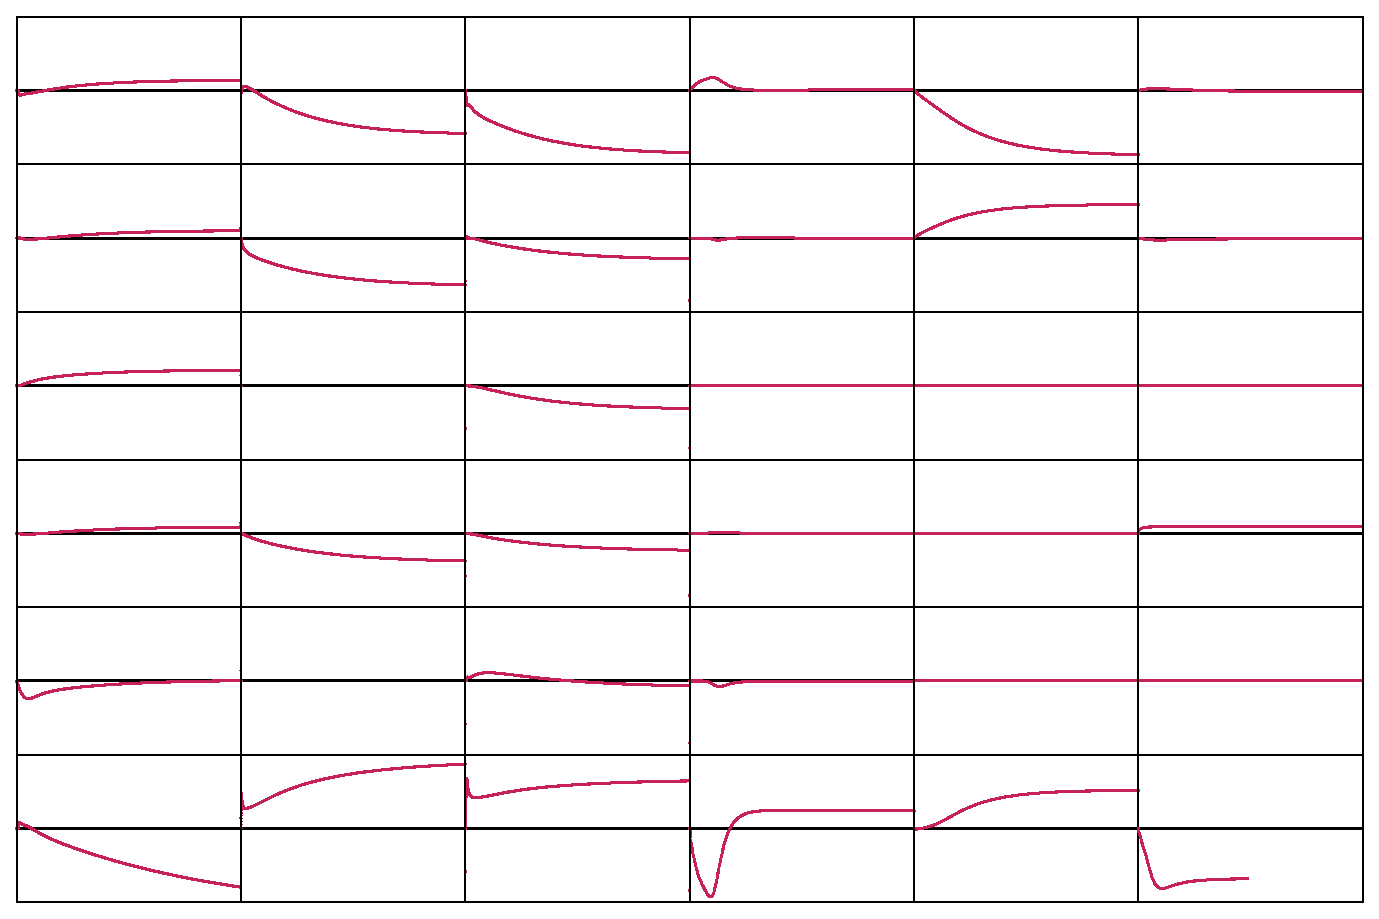
\includegraphics{GNUPlot/B1_Plot}}%
    \gplfronttext
  \end{picture}%
\endgroup

                    \caption{step responses.}
                    \label{fig:opt:stepresp}
                \end{figure}
            \end{landscape}

        \subsubsection{Dynamic profiles}
            The previous section showed only minor reactions to step changes in the manipulated variables. However
            a closer look at the dynamic column profiles reveals a much different picture. To analyze the internal
            column behaviour a external disturbance to the feed pressure was applied. As a result, the concentration
            profiles within the column undergo various changes. Especially with high purity separation sequences,
            a highly non-linear behaviour with two distinct characteristics is displayed. For one, two time scales can
            be observed, in which new steady states are reached. Secondly, the transition time
            between two steady states relies heavily on direction and magnitude of the disturbance \cite{Hwang.1991}.
            The first effect deals with short- and long-term dynamics, while the second is referred to as asymmetric dynamics.

            \begin{figure}
                \scriptsize
                \center
                \begin{subfigure}{0.48\textwidth}
                    \input{GNUPlot/N2_ADyn_plus}
                    \caption{Dynamic profile after feed enthalpy increase.}
                    \label{fig:N2_ADyn_plus}
                \end{subfigure}
                    \begin{subfigure}{0.48\textwidth}
                    \input{GNUPlot/N2_ADyn_minus}
                    \caption{Dynamic profile after feed enthalpy decrease.}
                    \label{fig:N2_ADyn_minus}
                \end{subfigure}
            \end{figure}

            From this preliminary study, of the dynamic process behaviour, it can be concluded, that an effective control strategy,
            should not only aim at directly maintaining the the product qualities, but rather to stabilize the internal column
            profiles. As the effects are often on time scales spanning over a day, there is a chance to detect malicious effects to
            product specifications in advance and and introduce appropriate counter measures. As can be seen in \figref{fig:N2_ADyn_plus}
            the external disturbance leads to formation of a concentration wavefront within the column. This behaviour is typical 
            for septation processes and be exploited to derive low-order models for control purposes \cite{Marquardt.1988}. 
            The fact that this non-linear behaviour is captured by the implemented models, further deepens the trust in the predictive
            capabilities of the implemented models. 








    \section{Model application issues}
            Aside from the actual model equations care must be taken as to how to implement any set of equations,
    such that a numerical solver can find feasible solutions. The most prominent issues one is faced with in
    that context are scaling and singularities within the model. Both aspects will be briefly discussed here.

        \subsection{Scaling}
        When evaluating a model, or integrating over a given time span, Taylor expansion is used to construct
        an approximate linear process model. This means, that a system of the form
        \Eq{eq:lin_sys}{
            \vec{A} x = b,
        }
        is solved to a specified absolute accuracy $\varepsilon$. For a single equation the choice of an appropriate
        value for $\varepsilon$ is rather simple, given that the magnitude of $\vec{A} x$ and $b$ is known.
        Here one needs to consider, that if either magnitude is much grater than $\varepsilon$ a large number
        of iterations will be necessary to solve the system in question. On the other hand, if they are of similar
        magnitude relative error in the attained solution might become unacceptably high.

        To address these issues it is wise to consider the model scaling while implementing the equations.
        One approach would be to introduce scaling factors on both sides of an equation. While this
        may certainly improve scaling for the equation itself, the opposite might be true for the respective derivative.
        Consider the following simple example \cite{MarkPinto.2008} where to holdups are added to a total holdup
        \Eq{}{
            f(M_i) = M_1 + M_2 = M_T
        }
        Assuming both holdups are of magnitude $M_1 = M_2 = 10^5kg$, then the function value is $2 \cdot 10^5$, while for
        the derivative
        \Eq{}{
            \fracddpart{f}{M_1} = \fracddpart{f}{M_2} = \fracddpart{f}{M_T} = 1
        }
        holds. Introducing a scaling factor of $10^{-5}$ to both sides of the equation would lead to a function value
        of $2$ but have an adverse effect on the derivatives $\fracddpart{f}{M_i} = 10^{-5}$.

        A more robust approach would be to scale the units of the given equation which can simultaneously improve
        scaling for the function and its derivatives. Writing the same equation in tonnes would lead to  function value of
        $200$ while maintaining the well scaled derivatives. Alternatively one can introduce further variables and equations
        with the aim to get more linear equation and rescale some parts of the original equation. A more linear function
        leads to more constant Jacobian elements and reduces the need for Jacobian updates which can be very expensive in
        computational terms.

        When it comes to the dynamic models, the issue of scaling is extend with another aspect. While for the steady-state
        models, one could rewrite each equation with different units, as long as each equation is in itself consistent,
        the same cannot be said, for the dynamic models. Here it is imperative, to maintain the same time scale for every
        dynamic equation. Due to the very large flow-rates, the steady-state and dynamic balances were written in
        $\frac{kmol}{hr}$ to achieve a well scaled equation. Considering the various dynamic effects discussed in
        the previous section, this seems to coarse to capture all relevant phenomena. Maintaining one time unit as one
        hour would lead to integrator steps of $\frac{1}{3600}$ for one second. Considering furthermore the small changes
        in the model variables, intuitively this would lead to very badly scaled problems. To somehow accommodate these
        considerations, it was decided, to introduce a scaling factor solely on the left hand side of the dynamic equations.
        By those means, the time scale of the process model can easily be adjusted for seconds, minutes, hours or days.

        \subsection{Singularities}
        Singularities in the models considered here often occur, when a variable is raised to a non-integer power,
        or the logarithm of a variable is evaluated.
        Expressions like have no solution within the rational domain, when the respective variable becomes negative.
        Furthermore when negative exponents are involved a value of zero would lead to a division by zero which is
        undefined. Even before that the function value might become very large as the variable approaches zero.

        In the context of a distillation column, this issue becomes especially relevant, when optimizations or simulations
        with inactive trays are carried out. Some flowrates in the inactive section of the model will be zero, depending
        on whether the top or bottom reflux is optimized, those will be either vapour or liquid flowrates. While a
        solution of zero might cause issues in some cases, a negative solution introduces even more complications. As the
        equations are solved within numerical accuracy, this might also lead to (slightly) negative solutions, which will
        cause the numerical solver to fail. Such scenarios have to be anticipated while implementing the model and
        appropriate measures have to be taken to ''protect'' such variables from hindering model evaluation.

        As \gproms supports state transition networks, one way is to introduce conditional statements. However
        those statements will in almost all cases lead to discontinuities in the model. While in principal such
        discontinuities can be detected by numerical solvers \cite{Pantelides.2003}, they are a further source
        for instabilities. Hence they should in the best case only be introduces, when there is a physical correspondence
        in the system behaviour.

        In this thesis the problem was approached by decoupling the flowrates within the column, and the ones used for evaluation
        of the hydraulic model. With the help of the split fractions active and inactive trays can be distinguished.
        \Eq{}{
            V_j^{\text{hyd}} = \left( \sum_{k=1}^j \zeta^R_k \right) \cdot V_j + \left(1 - \left( \sum_{k=1}^j \zeta^R_k \right)\right) \cdot V_1
        }
        Here it should be pointed out, that it only needs to be ensured, the the hydraulic model can be evaluated for inactive trays.
        What results are returned for these trays has no effect for the modelled column operation.
        
        \subsection{Time scale}
        The discussion of the dynamic column behaviour revealed, that dynamic effects are occurring on very different time scales. 
        Some are to the order of seconds, others hours and days. Naturally, the finest scale determines the required accuracy. 
        However a very high accuracy leads to an excessive amount of computational time as the model has to be evaluated 
        much more often, as the resolution of the discredited time increases. Furthermore the aspect of model scaling 
        once more has to be considered. As said before, scaling of units is the most effective way, to both scale equations 
        and derivatives. In the case of the ASU process, kmol/hr was selected for the material balances. Hence the 
        dynamic terms are also in terms of hours. This is way too coarse for the purposes of studding the dynamic 
        behaviour. However rewriting the equation in seconds would lead to a (in this particular case) badly scaled equation. 
        In order to retain the well-scaled equation and increase the resolution, a scaling factor for the dynamic terms was 
        introduced, by which the time scale of the terms was adjusted to seconds. As a side effect, the time scale can be 
        easily adjusted to cater to the specific needs in a simulation. Arguably, there are some issues with accuracy, using the 
        given approach, as in fact the convergence accuracy is reduced to the order of the scaling factor. However it was 
        found to be the most promising solution given the tradeoff between model accuracy and robustness. 

